\documentclass[margin=2mm]{standalone}
\usepackage{tikz}
\usetikzlibrary{calc}
\usetikzlibrary{patterns}
\usetikzlibrary{decorations.text}
\usetikzlibrary{decorations.pathmorphing}
\usetikzlibrary{decorations.markings}

\begin{document}

\begin{tikzpicture}

\node [inner sep=0pt,above right] (ab) {
    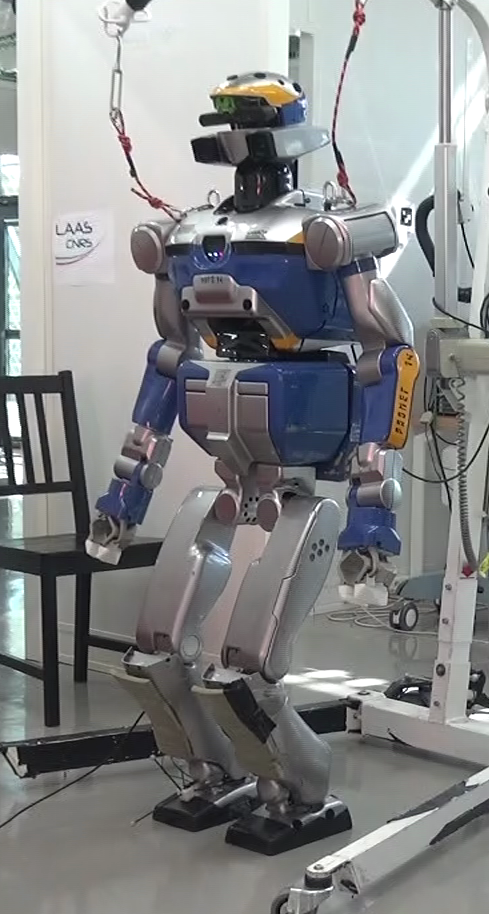
\includegraphics[width=9cm]{HRP2-setup.png}
};

\node [inner sep=0pt,] at (12.0,15.0) (flmone) {
    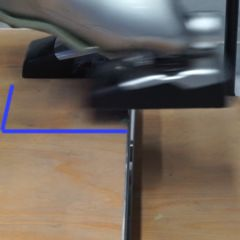
\includegraphics[width=3cm]{feet_landing_mark_1.jpg}
};


\node [inner sep=0pt] at (12.0,11.0) (flm2) {
    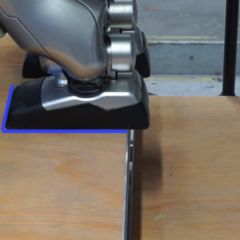
\includegraphics[width=3cm]{feet_landing_mark_2.jpg}
};

\node [inner sep=0pt] at (17.0,10.0) (mc) {
    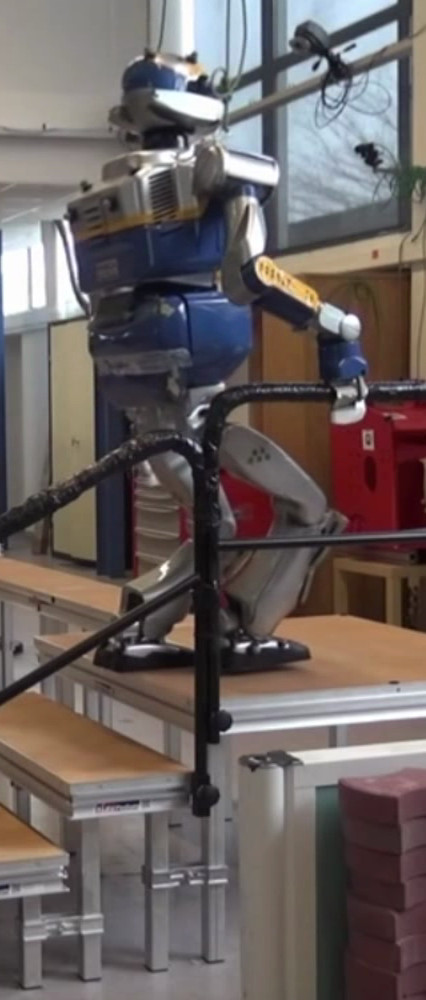
\includegraphics[width=4cm]{HRP2-multicontacts.jpg}
};

\node [inner sep=0pt] at (12.0,7.0) (flm4) {
    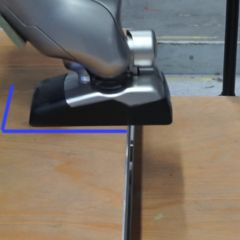
\includegraphics[width=3cm]{feet_landing_mark_4.jpg}
};

\node [inner sep=0pt] at (12.0,3.0) (flm5) {
    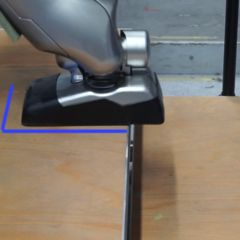
\includegraphics[width=3cm]{feet_landing_mark_5.jpg}
};

%% \node [inner sep=0pt] at (12.0,0.0) (flm6) {
%%     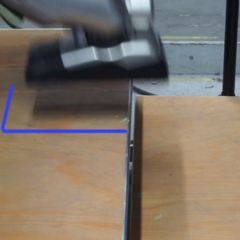
\includegraphics[width=3cm]{feet_landing_mark_6.jpg}
%% };

\node[below=0.1cm] at (flmone.south) (a) {(a)};
\node[below=0.1cm] at (flm2.south) (b) {(b)};
\node[below=0.1cm] at (flm4.south) (c) {(c)};
\node[below=0.1cm] at (flm5.south) (d) {(d)};
%\node[below=0.1cm] at (flm6.south) (e) {(e)};
\node[below=0.1cm] at (mc.south) (e) {(e)};

%\draw[step=1.0,black,thin](0.0,-0.0) grid (20.0,17.0);


\def\cosyaxis{0.866025403784}
\def\sinyaxis{-0.5}
\def\cosxaxis{-0.866025403784}
\def\sinxaxis{-0.5}
\def\coszaxis{-0.34202}
\def\sinzaxis{0.93969}

% define IMU Frame
\coordinate (cos_ori) at (3.4, 2.2);
%\fill[magenta] (cos_ori) circle (2pt); % show origin

\def\ax_length{1.5}
\path (cos_ori) ++ ( \ax_length * \cosxaxis, \ax_length * \sinxaxis) coordinate (cos_x);
\def\ax_length{1.0}
\path (cos_ori) ++ ( \ax_length * \cosyaxis, \ax_length * \sinyaxis) coordinate (cos_y);
\def\ax_length{1.5}
\path (cos_ori) ++ ( \ax_length * \coszaxis, \ax_length * \sinzaxis) coordinate (cos_z);

\draw [->, very thick, blue!70] (cos_ori) -- (cos_x);
\draw [->, very thick, blue!70] (cos_ori) -- (cos_y);
\draw [->, very thick, blue!70] (cos_ori) -- (cos_z);

\node[draw=none,text=blue!70, above left]  at (cos_ori) {$\mathcal W_{IMU}$};

\coordinate (right_ankle) at (4.3,2.6);
\coordinate (right_knee) at (3.0,5.0);
\coordinate (right_hip_pitch) at (3.7,7.7);
\coordinate (right_hip_roll) at (4.5,7.5);
\coordinate (right_hip_yaw) at (4.5,8.5);

\coordinate (left_hip_yaw) at (5.3,8.5);
\coordinate (left_hip_roll) at (5.3,7.5);
\coordinate (left_hip_pitch) at (5.5,7.5);
\coordinate (left_knee) at (4.3,4.6);
\coordinate (left_ankle) at (5.7,2.3);


\draw [very thick, brown!70] (right_ankle) -- (right_knee);
\draw [very thick, brown!70] (right_knee) -- (right_hip_pitch);
\draw [very thick, brown!70] (right_hip_pitch) -- (right_hip_roll);
\draw [very thick, brown!70] (right_hip_roll) -- (right_hip_yaw);
\draw [very thick, brown!70] (left_hip_yaw) -- (right_hip_yaw);
\draw [very thick, brown!70] (left_hip_yaw) -- (left_hip_roll);
\draw [very thick, brown!70] (left_hip_roll) -- (left_hip_pitch);
\draw [very thick, brown!70] (left_ankle) -- (left_knee);
\draw [very thick, brown!70] (left_knee) -- (left_hip_pitch);


\end{tikzpicture}

\end{document}
